\documentclass[a4paper, 11pt, french]{article}

\usepackage[french]{babel}
\usepackage[utf8]{inputenc}
\usepackage[T1]{fontenc}
\usepackage{csquotes}
\usepackage{amsmath,amsfonts,amssymb,mathrsfs}
\usepackage[includeheadfoot, hmargin=2cm, top=0.9cm, bottom = 1.8cm, headsep=2cm]{geometry}
\usepackage{lmodern} %pas pixelisé
\usepackage{engrec,titlesec,lipsum,xcolor}
\usepackage{fancybox}
\usepackage[skins, most]{tcolorbox}
\usepackage[bookmarks={true},bookmarksopen={true}, pdftitle={Cahier des charges}, pdfauthor={Chevalier Romain}, pdfsubject={Caméra domes}, hidelinks]{hyperref}
\usepackage{setspace}
\usepackage{stmaryrd}
\usepackage{multicol} 
\usepackage{enumitem}
\usepackage{array,multirow,makecell}
\usepackage{titlesec}
\usepackage{multirow}
\usepackage{hyperref}
\usepackage{listings}
\usepackage{graphicx}
\usepackage{caption}
\usepackage{subcaption}
\usepackage{float}
\usepackage{fancyhdr}
\usepackage[bottom]{footmisc}
\usepackage{footnote}
\usepackage[page,header]{appendix}
\usepackage{titletoc}
\makesavenoteenv{tabular}
\makesavenoteenv{table}

\graphicspath{{Figures/}{Photos/}}

\usepackage{tikz}
\usepackage{pgfplots}
\pgfplotsset{compat=1.18} 
\usetikzlibrary{decorations.pathmorphing, shapes, automata,positioning}



%-----------------------------------------------------------------------------------

\pagestyle{fancy}
\renewcommand{\headrulewidth}{1pt}
\fancyhead[C]{\leftmark} 
%\fancyhead[R]{\includegraphics[scale=0.13]{logoAdeoService.jpg}}
\fancyhead[R]{
\includegraphics[scale=0.1]{Logo_CENTRALE_C.png}}
\newcolumntype{M}{>{\centering\arraybackslash}m{1.75cm}}
\setlength{\headheight}{30.5pt}

%-----------------------------------------------------------------------------------

\frenchbsetup{StandardLists=true}
%\setlength{\parskip}{1em}
\AddThinSpaceBeforeFootnotes
\FrenchFootnotes

%---------------------------------------------------------------

%-----------------------------------------------------------------------------------

\definecolor{vert}{rgb}{0,0.69,0.31}
\definecolor{bleue}{rgb}{0,0.31,0.69} 
\definecolor{violet}{rgb}{0.38,0.18,055} % 97, 45, 140     244, 208, 63
\definecolor{jaune}{rgb}{0.96, 0.85, 0.23}

\definecolor{darkWhite}{rgb}{0.94,0.94,0.94}
\definecolor{vert}{rgb}{0,0.69,0.31}
\definecolor{rose}{rgb}{1,0.08,0.58}% rgb(255,20,147)
\definecolor{rouge}{rgb}{0.78,0.12,0.08}
\definecolor{gris}{rgb}{0.4,0.4,0.4}
\definecolor{marron}{rgb}{0.4,0.2,0}
\definecolor{darkWhite}{rgb}{0.94,0.94,0.94}

%-----------------------------------------------------------------------------------

\title{%
        \Huge Suivi d'un grimpeur par caméra dome \\
        \LARGE Cahier des charges}

\author{\LARGE CHEVALIER Romain}
\date{\today}

\newcommand{\hsp}{\hspace{20pt}}
\newcommand{\HRule}{\rule{\linewidth}{0.5mm}}

%-----------------------------------------------------------------------------------

\newcounter{obj}
\setcounter{obj}{1}


%-----------------------------------------------------------------------------------


\begin{document}
\pagenumbering{roman}
\begin{titlepage}

    \begin{titlepage}
        \begin{center}
      
          % Upper part of the page. The '~' is needed because \\
          % only works if a paragraph has started.
      
          \textsc{\LARGE École Centrale De Lille}\\[2cm]
      
          \textsc{\huge Projet d'intégration}\\[2cm]
      
          % Title
          \HRule \\[0.4cm]
          { \Huge \bfseries Suivi d'un grimpeur par caméra dome\\[0.4cm] }
      
          \HRule \\[2cm]

          \textsc{\Large Cahier des charges\\} {\large\today}\\[1.5cm]
          
          \vfill
      
          % Author and supervisor
          \begin{minipage}{0.4\textwidth}
            \begin{flushleft} \large
              CHEVALIER Romain\\
            \end{flushleft}
          \end{minipage}
          \begin{minipage}{0.4\textwidth}
            \begin{flushright} \large
              \emph{Tuteur :}  BOURDEAUD'HUY T. \\
            \end{flushright}
          \end{minipage}
      
          \vspace{1cm}
         
        \end{center}
      \end{titlepage}
    
    \normalsize
   
\end{titlepage}

%-----------------------------------------------------------------------------------

\setcounter{secnumdepth}{3}
\setcounter{tocdepth}{3}
\startcontents[sections]

%-----------------------------------------------------------------------------------
\tableofcontents
%\printcontents[sections]{l}{1}{\setcounter{tocdepth}{3}}
%\printcontents[sub]{l}{1}{\setcounter{tocdepth}{2}}
\pagenumbering{arabic}
\newpage

%-------------------------------------------------------------

\section{Contexte}
Afin d'améliorer les services offerts aux utilisateurs d'une salle d’escalade, on envisage de mettre en place un système de suivi automatisé des grimpeurs à l'aide de caméras IP dômes motorisées. Ces caméras permettront de suivre les mouvements des grimpeurs sur les différentes voies en ajustant automatiquement le cadrage et le zoom en fonction de leur position. Cette solution vise à offrir un support d'analyse post-session, afin de permettre aux grimpeur de comprendre leurs forces et faiblesses pour s'améliorer.

Le système proposé sera composé de trois éléments principaux, voir schéma en figure~\ref{fig:archiMat} :
\begin{itemize}
  \item \textbf{Deux caméras IP dômes motorisées}\footnote{Caméra réseau à dôme AXIS COMMUNICATION - Q6034-E, voir \href{https://www.axis.com/dam/public/11/e4/20/cam\%C3\%A9ra-r\%C3\%A9seau-\%C3\%A0-d\%C3\%B4me-ptz-axis-q6034-e-fr-FR-201515.pdf}{fiche technique}.} qui permettront le suivi en temps réel des grimpeurs.
  \item \textbf{Un serveur} chargé de la capture des flux vidéo, du stockage des enregistrements et du maintien d’une base de données associée aux vidéos.
  \item \textbf{Une interface utilisateur sur tablette} pour configurer et lancer de nouveaux enregistrements, consulter les vidéos en direct ou enregistrées et paramétrer le système.
\end{itemize}

\begin{figure}
  \centering
  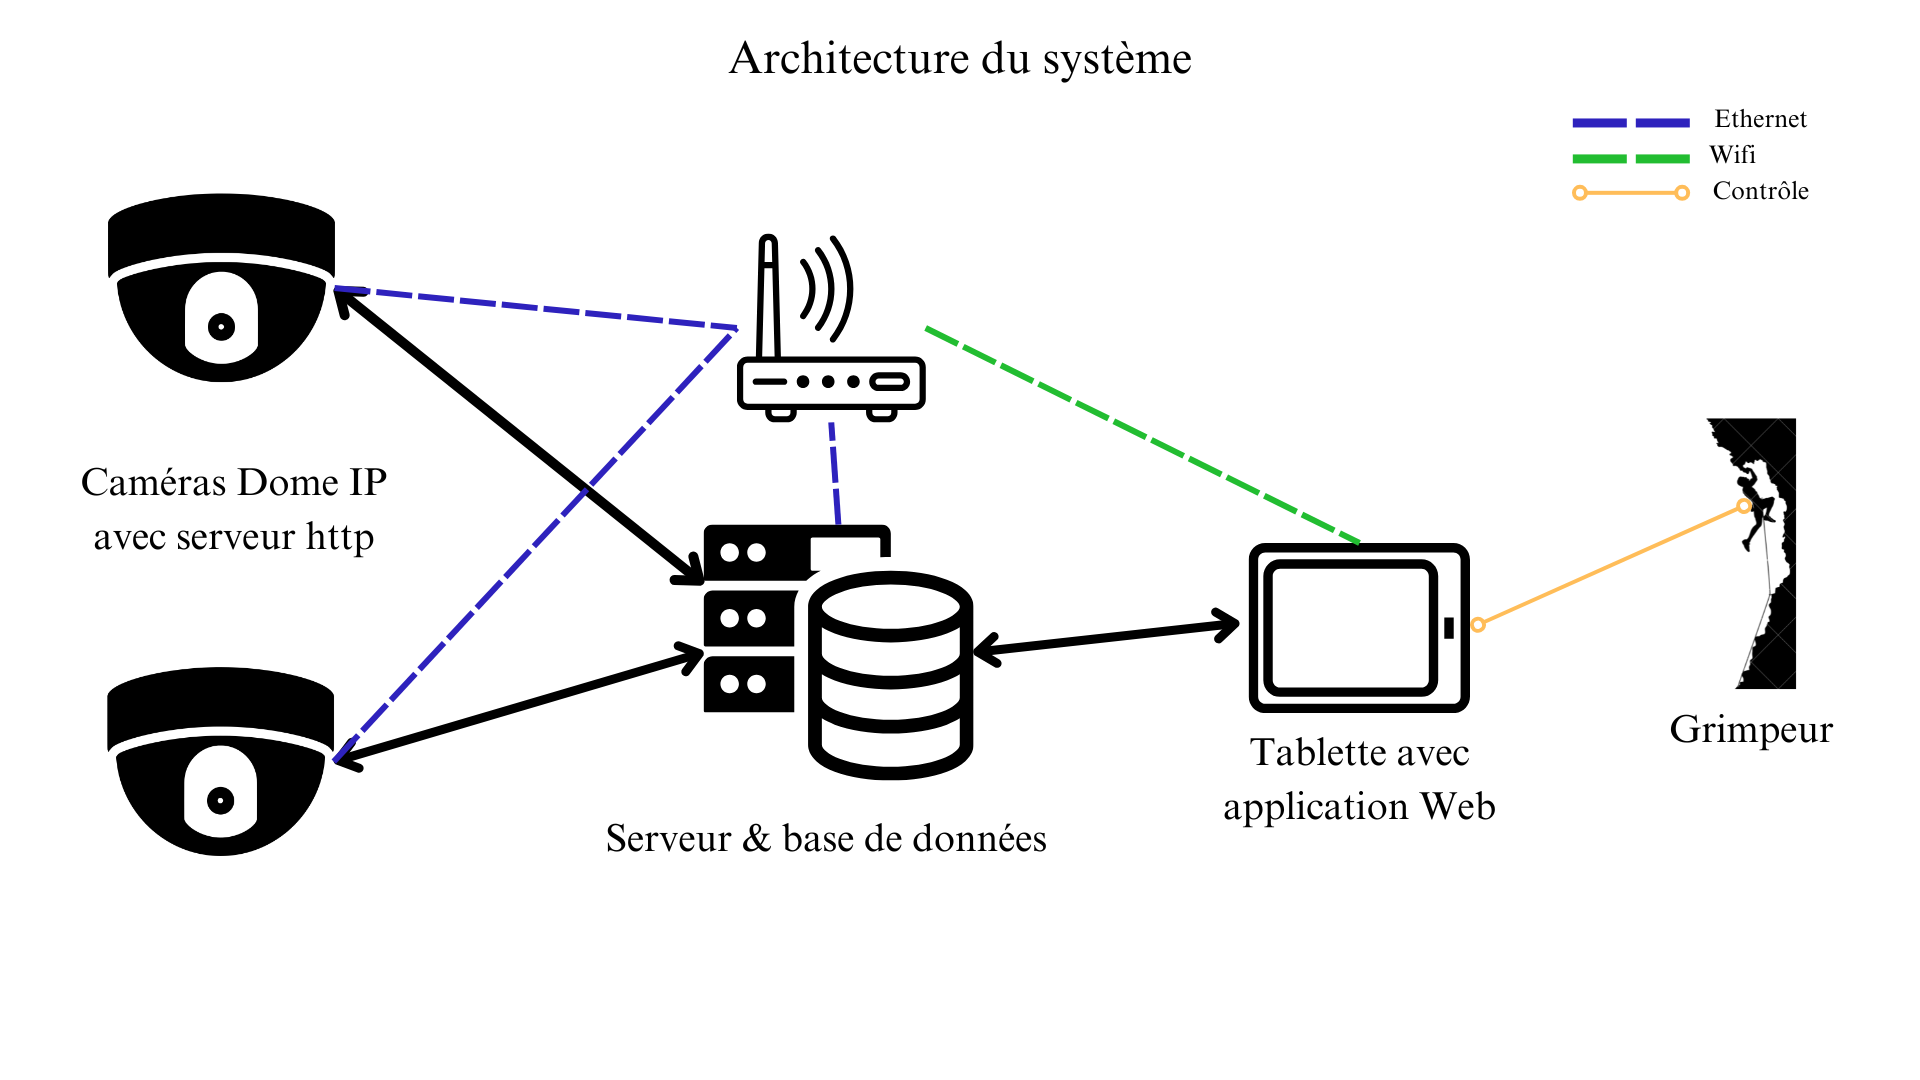
\includegraphics[width=.8\textwidth]{Architecture.png}
  \caption{Architecture matérielle du système envisagée}
  \label{fig:archiMat}
\end{figure}

\section{Objectifs}
\subsection{Caméra}
Afin de réaliser le projet, je dispose de deux caméras domes IP PTZ\footnote{Pan Tilt Zoom en français: panoramique, inclinaison et zoom} Q6034-E provenant d'\textit{AXIS COMMUNICATION}. Les caméras créent un serveur HTTP en local permettant de visualiser le flux de données en direct, de piloter la caméra et de la paramétrer. Elle possède déjà une option de suivi automatique des personnes, il s'agira de s'assurer que la camera prend bien le focus sur le grimpeur et non l'assureur au démarrage. 

\begin{figure}
  \centering
  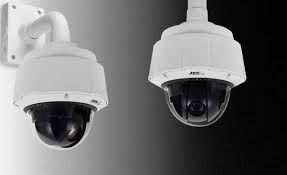
\includegraphics[]{cameraQ6304.jpg}
  \caption{Caméra réseau à dôme PTZ AXIS Q6034-E - \textit{AXIS COMMUNICATION}}
\end{figure}


\paragraph*{Objectif \theobj : } Être capable de streamer le flux video et de recevoir des ordres de pilotage par le serveur et la tablette. La caméra doit aussi être configurable par le serveur.

\paragraph*{Objectif \stepcounter{obj}\theobj : } Suivre le grimpeur lors de la montée, de la descente ou lors d'une chute.


\subsection{Serveur}
Le serveur joue un rôle central dans cette architecture, il va permettre d'enregistrer et de stocker les vidéos des grimpeurs. Il contiendra aussi une base de données afin de pouvoir associer les vidéos à différentes données (voir paragraph suivant). Le serveur devra êre accessible par wifi depuis la tablette afin de visualiser les vidéos.

\paragraph*{Objectif \stepcounter{obj}\theobj.1} Enregistrer et stocker les vidéos sur un serveur.
\paragraph*{Objectif \theobj.2} Mise en route automatique de l'enregistrement lorsque le grimpeur démarre.

\paragraph*{Base de données}
Chaque vidéo sera référencée par un numéro de voie, un nom et prénom de grimpeur, une difficulté de voie et le type de grimpe (moulinette ou tête) et la date du jour et l'heure de début d'enregistrement. Cela permettra de facilement retrouver la vidéo. 

\paragraph*{Objectif \stepcounter{obj}\theobj} Être capable de retrouver une vidéos avec seulement quelques infos. 

\subsection{Interface utilisateur sur tablette\label{sec:UX}}
Pour faciliter l'utilisation des caméras, une tablette permettra de les exploiter. Elle servira entre autre à lancer un enregistrement et à regarder les vidéos enregistrées pour les analyser, voir maquette de l'application en figure~\ref{fig:mockup}. Sur l'écran pour lancer l'enregistrement (voir figure~\ref{fig:nvEnreg}), il sera possible même lorsque l'enregistrement sera lancé de passer en mode manuel et faire son propre tracking. Et inversement, on pourra passer en mode de tracking automatique. 

\paragraph*{Objectif \stepcounter{obj}\theobj} Communiquer avec le serveur pour lancer, visionner, télécharger et partager des enregistrements.

\paragraph*{Objectif \stepcounter{obj}\theobj} Piloter la caméra depuis la tablette. 

\begin{figure}[!ht]
  \centering
  \begin{subfigure}[c]{.48\textwidth}
    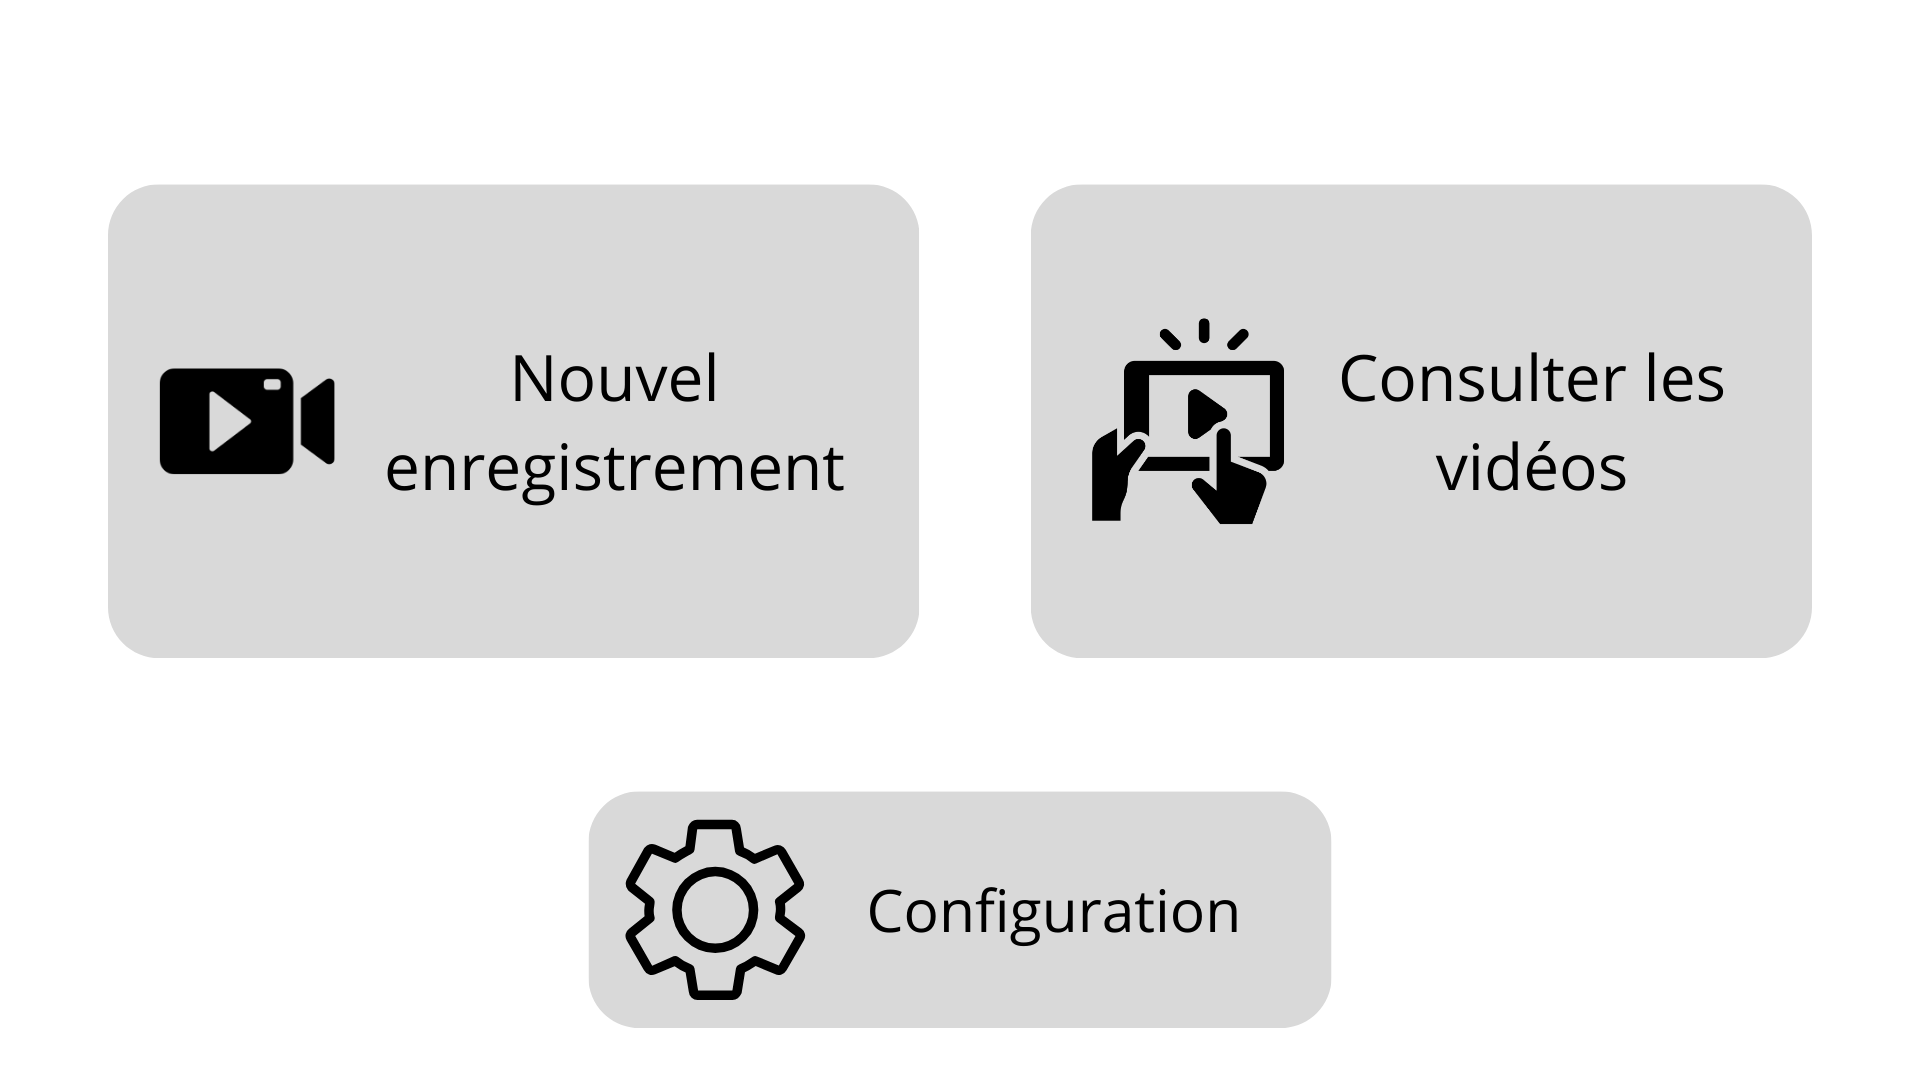
\includegraphics[width=\textwidth]{Ecran accueil appli.png}
    \caption{Page d'accueil de l'application}
  \end{subfigure}
  \begin{subfigure}[c]{.48\textwidth}
    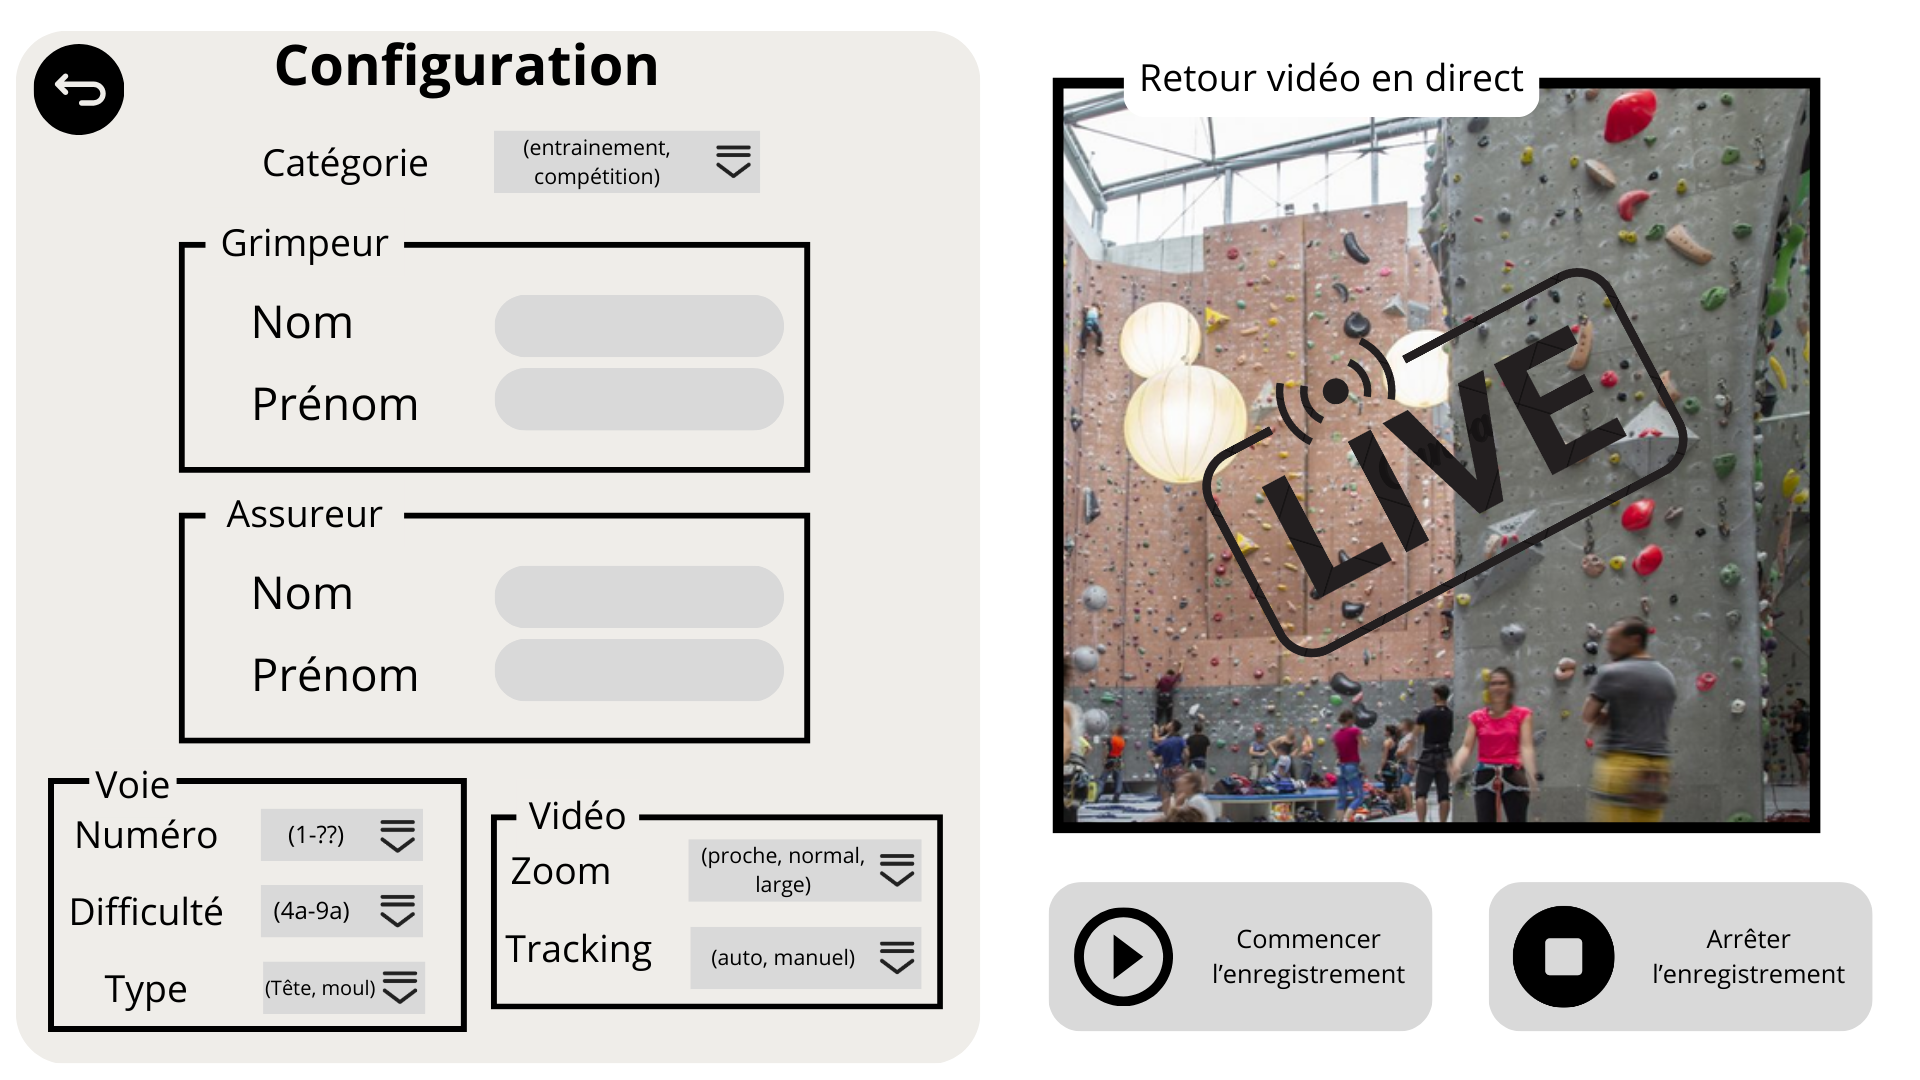
\includegraphics[width=\textwidth]{Nouvel enrgistrement.png}
    \caption{Nouvel enregistrement}
    \label{fig:nvEnreg}
  \end{subfigure}

  \begin{subfigure}[c]{.48\textwidth}
    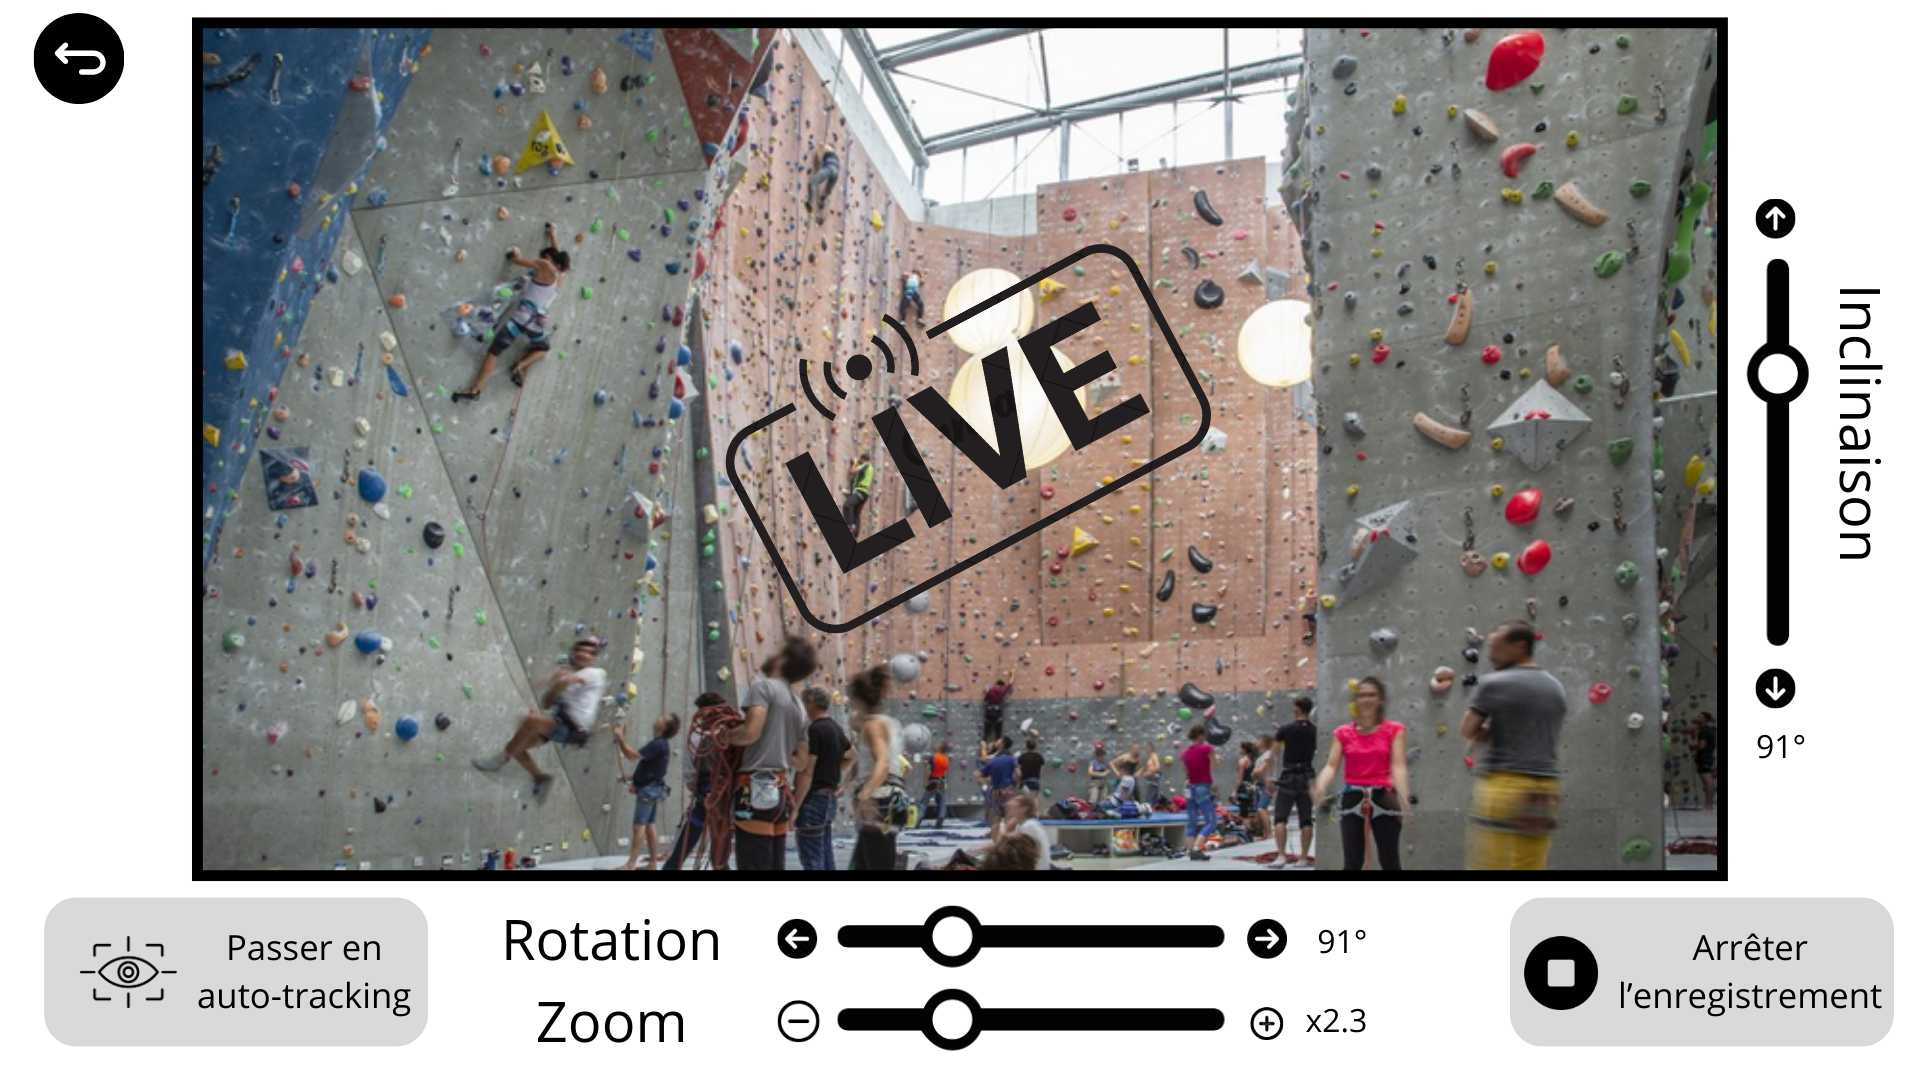
\includegraphics[width=\textwidth]{Tracking manuel.png}
    \caption{Tracking manuel}
  \end{subfigure}
  \begin{subfigure}[c]{.48\textwidth}
    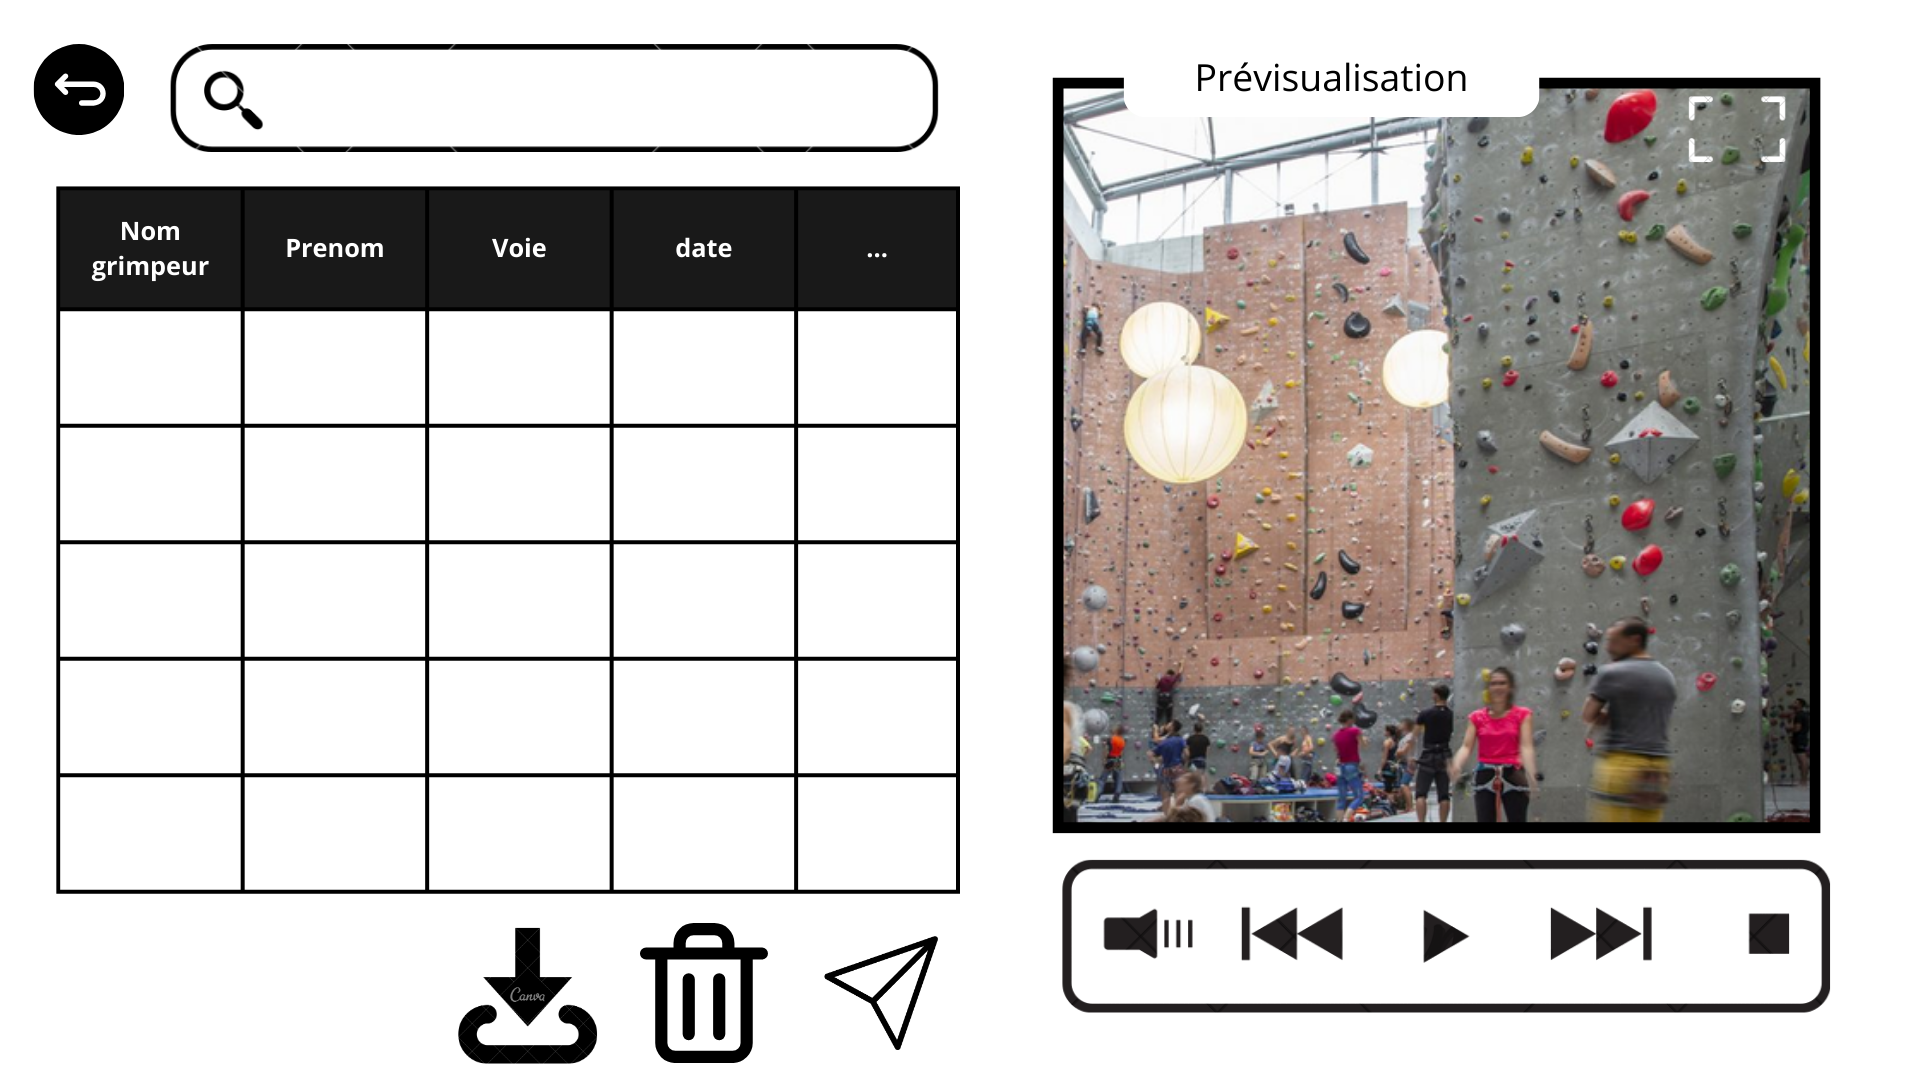
\includegraphics[width=\textwidth]{Consultation videos.png}
    \caption{Consultation vidéos}
  \end{subfigure}

  \begin{subfigure}[c]{.48\textwidth}
    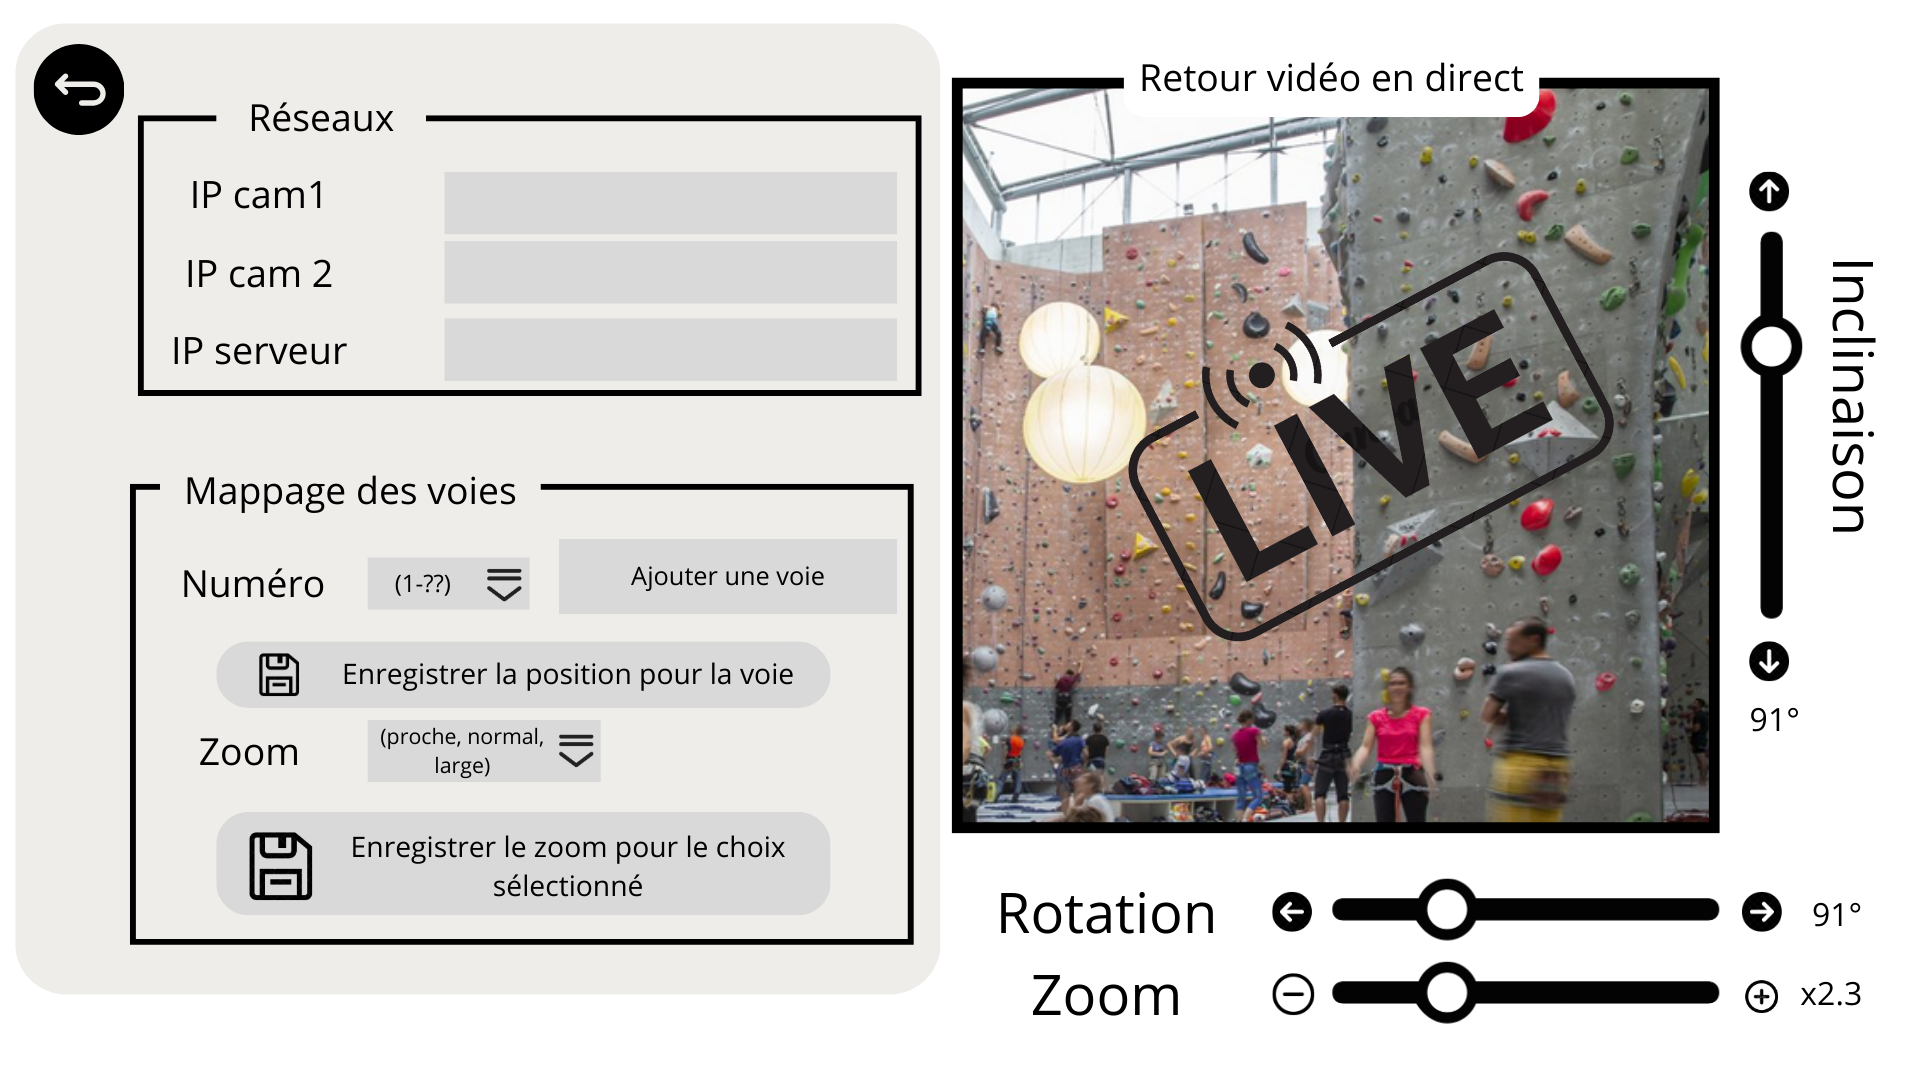
\includegraphics[width=\textwidth]{Reglages.png}
    \caption{Réglages de l'application}
  \end{subfigure}
  \caption{Mock up de l'interface utilisateur}
  \label{fig:mockup}
\end{figure}

\section{Périmètre}

Le périmètre de ce projet couvre l'ensemble des éléments techniques et fonctionnels nécessaires à la mise en place d'un système automatisé de suivi des grimpeurs dans une salle d'escalade. Il s'agit notamment de :

\begin{itemize}
  \item \textbf{Installation des caméras IP dômes motorisées} Le projet inclut l'intégration et la configuration de deux caméras permettant de suivre les grimpeurs en temps réel en ajustant automatiquement le zoom et l'orientation en fonction de leur position.
  \item \textbf{Mise en place du serveur} Le serveur sera responsable de la gestion des flux vidéo, de leur enregistrement et du stockage des vidéos dans une base de données. Il devra également être capable de gérer les paramètres des caméras et de fournir un accès aux vidéos enregistrées via un réseau Wi-Fi.
  \item \textbf{Développement de l'interface utilisateur} Une interface intuitive sur tablette permettra de piloter les caméras, de lancer des enregistrements, d'accéder aux vidéos en direct et enregistrées, et de configurer les options du système.
\end{itemize}


Le projet s'inscrit dans un cadre d'intégration technologique visant à améliorer l’expérience utilisateur et à offrir des outils de suivi et d'analyse performants pour les grimpeurs.
  
\section{Description fonctionnelle des besoins}

Le projet vise à fournir une solution automatisée de suivi et d’enregistrement des grimpeurs dans une salle d'escalade en utilisant des caméras IP motorisées, un serveur central et une interface utilisateur sur tablette. Voici les besoins fonctionnels principaux :

\begin{itemize}
    \item \textbf{Caméras IP motorisées} : Les caméras doivent pouvoir suivre les grimpeurs en temps réel, ajuster automatiquement leur cadrage et zoom en fonction des mouvements des grimpeurs. Elles doivent également être configurables via le serveur pour permettre le streaming et la réception d’ordres de pilotage depuis la tablette.
    
    \item \textbf{Serveur centralisé} : Le serveur joue un rôle clé dans la gestion du flux vidéo. Il sera responsable de :
    \begin{itemize}[label=$-$]
        \item L’enregistrement et le stockage des vidéos capturées par les caméras.
        \item La gestion d’une base de données associant chaque vidéo à des informations spécifiques telles que le grimpeur, l’assureur, la difficulté de la voie, et la date. Cette base de données facilitera la recherche et l’accès aux enregistrements.
        \item La communication avec l’interface utilisateur pour permettre le contrôle des caméras et l’accès aux vidéos enregistrées.
        \item Cryptage des vidéos et données sur les utilisateurs (Non prioritaire)
    \end{itemize}
    
    \item \textbf{Interface utilisateur sur tablette} : L’interface doit permettre aux utilisateurs de :
    \begin{itemize}
        \item Configurer et piloter les caméras, notamment en basculant entre le mode automatique (tracking) et manuel.
        \item Lancer de nouveaux enregistrements.
        \item Visualiser les vidéos en direct ou consulter les vidéos enregistrées pour analyse.
        \item Personnaliser les paramètres du système selon les besoins des grimpeurs et des gestionnaires de la salle.
    \end{itemize}
\end{itemize}

Chaque composant du système doit fonctionner de manière fluide pour garantir une expérience utilisateur optimale, avec des fonctionnalités avancées de suivi automatisé des grimpeurs.


\section{Délais}
Le projet de mise en place du système de suivi des grimpeurs doit être réalisé et terminé d'ici mars 2025. Voici les principaux jalons: 
\begin{itemize}
  \item \textbf{Fin novembre} Serveur et base de donnée crées et le serveur est capable d'enregistrer des vidéos. 
  \item \textbf{Mi janvier} Première ébauche de l'application permettant de consulter les vidéos sur le serveur. 
  \item \textbf{Fin février} Application sur la tablette fonctionnelle.
  \item \textbf{Mars} Réalisation de tests fonctionnels ajustements nécessaires.
\end{itemize}






%-----------------------------------------------------------
% \clearpage
% \newpage


% \section*{Annexes}
% \addcontentsline{toc}{section}{Annexes}

% \appendix

% \startcontents[sections]
% \printcontents[sections]{l}{1}{\setcounter{tocdepth}{2}}


%     \section{Glossaire}
      




\end{document}